\documentclass[10pt,conference,compsocconf]{IEEEtran}

\usepackage{hyperref}
\usepackage{graphicx}	% For figure environment
\usepackage[table,xcdraw]{xcolor}
\usepackage{pgfplots}



\begin{document}
\title{Machine Learning for Discovering the Higgs Particle}

\author{
  David Alonso del Barrio, Francisco Javier Blázquez Martínez, Andrés Montero Ranc\\
  \textit{Department of Computer Science, EPFL, Switzerland}
}

\maketitle

\begin{abstract}
Machine Learning techniques are increasingly popular today and are used in several fields of science. These techniques are useful when dealing with complex and large data sets,  which sometimes represent the result of scientific experiments. In this project we implement some of the most popular methods, applying them to a data-set from CERN, to solve a binary classification problem.
\end{abstract}

\section{Introduction}

This project aims to find the best binary classification method to distinguish Higgs Boson signals from background noise and use these results to predict the correct label for each new observation. We used a CERN's labeled data set containing up to thirty different features measurements for 250.000 collisions in the Large Hadron Collider. First, we had to clean up this huge amount of data, facing outliers, missing values, discrete variables... Then we proceeded to train models based on Linear Regression, Ridge Regression, Logistic Regression, Regularized Logistic Regression and, of course, the measure of their behaviour and accuracy.

\section{Data Preprocesing}
For our models (specially for Linear regression with least squares loss function and its regularization) the best and almost only way to improve our model's accuracy was by data preprocessing.

\subsection{Features analysis}
We first analyzed the features and checked that \textit{pri\_jet\_num} is a categorical variable (values in \{0,1,2,3\}) and that some features had a huge amount of missing values. We decided not to split our data by \textit{pri\_jet\_num} because when training models for this splitted data the weighted (in data size) average of the accuracies wasn't improving our model.

\subsection{Dropping features}
Since some features had more than 70\% of missing values, it's reasonable to think they could be adding more noise than useful data, we implemented a method for dismissing features with missing values frequency greater than a given threshold (MVT). We also implemented a method for removing features with Pearson's correlation coefficient greater than a threshold (CT).

\subsection{Missing values management}
Removing all features with missing values made us losing accuracy because we lost much information. We tried then to keep some of these and replace the missing values by zero (for positive features, less deviated than -999) or by the mean of the valid measurements.

\subsection{Outliers}
Some features had data with values more than a hundred times the standard deviation distance from the mean, we also tried removing points with values deviated more than a threshold (OT).

\subsection{Standarization of data}
We have tried two types of feature standardization, Z standardization, and max-min standardization, but we have opted for the first one because we have seen better results.

\subsection{Increase regresion order}
 We created artificial features from the original data to work with a more expressive model. Adding the product of every pair of features helped us reaching a higher precision. We tried adding also features raised up to certain exponent (AD).

\section{Cross Validation}
We have described some hyper parameters for our data preprocessing, these, along with the regression model parameters fully determine our model. We used cross-validation to chose the best parameters, this is, find the best models. 

Concretely, we did a grid search for every model with 5 folds cross-validation to have a faster computation and find the approximate good candidates for the parameters. Once we found good candidates, we further refined the search by increasing it to a 10 folds cross-validation. With this approach, for reaching an optimal point we had to do several steps each one with a different (and random) split of the data set for the cross validations so we didn't consider necessary analyzing also the deviation of the values during the cross validation.

We now describe the best parameters and accuracies obtained for every model.

\section{METHODS AND MODELS}

\subsection{Linear regression using Gradient Descent and Stochastic Gradient Descent} 
Since we had enough train data, overlearning wasn't a problem (in that situation these models could have been better than other approaches) and these models obtained always a worse accuracy than \textit{least squares}. However, both worked well and we were able to obtain a \textbf{0.745} precission.

\subsection{Least squares}
For least squares we obtained a \textbf{0.804} precission with MVT=1, CT=0.925, OT=11, AD=4. Surprisingly, without removing the features with 70\% of missing values and not considering outliers points deviated up to 11 times the standard deviation from the mean.

\subsection{Ridge Regression}
We obtained our best model with ridge regression. We obtained a \textbf{0.81} precission with MVT=1 CT=1 OT=10 AD=4, LAMBDA=11;. Surprisingly again, without removing the features with 70\% of missing values and without removing neither correlated features and being lax with outliers.

\subsection{Logistic Regression}
A precission \textbf{0.752} was obtained for the following parameters MVT=1 CT=1 OT=6 AD=2 GAMMA=1e-06. However it didn't react well to feature augmentation.

\subsection{Regularised Logistic Regression}.
The optimum parameters to reach the maximum accuracy for our model were MVT=10; CT=0.85; OT=8; AD=8; LAMBDA=1; GAMMA=1e-07 for which we obtained an accuracy of \textbf{0.7926}. Both in this case and in logistic regression they required a lot of computation time, we wasn't able to test lower gammas and increasing the maximum number of iterations more than 10000.

\section{Conclusions}
Surprisingly, in most algorithms, eliminating features with many missing values has had a negative impact. 

Best results have been obtained using Ridge Regression algorithm with a lamba equal to 11, without feeding missing values, nor correlated characteristics, and eliminating very few outliers. We tried to play with the Lamba values and with the augmentation degree, discovering that if we used a bigger Lamba we could increase the degree and improve the accuracy.


The best result was achieved using the Ridge Regression algorithm. However, an essential step was the pre-processing of data since no model exceeded 74\% accuracy without it. With a degree of 4 for polynomial terms, the maximum accuracy reached was \textbf{81\%}. To expand our work further we could try neural network algorithms.



\begin{table}[]
\centering
\begin{tabular}{|l|l|l|l|l|l|}
\hline
Precision                       & MVT & CT                           & OT                          & AD                        & LAMBDA                       \\ \hline
0.789616                        & 1   & \cellcolor[HTML]{FFCCC9}0.85 & 7.5                         & 2                         & 0.01                         \\
0.793268                        & 1   & \cellcolor[HTML]{FFCCC9}1    & \cellcolor[HTML]{C3DCFF}7.5 & 2                         & 0.01                         \\
0.797484                        & 1   & 1                            & \cellcolor[HTML]{C3DCFF}9   & 2                         & 0.01                         \\
0.798116                        & 1   & 1                            & \cellcolor[HTML]{C3DCFF}10  & 2                         & \cellcolor[HTML]{BFDEBF}0.01 \\
0.799060                        & 1   & 1                            & 10                          & \cellcolor[HTML]{FFFC9E}2 & \cellcolor[HTML]{BFDEBF}0.1  \\
0.803928                        & 1   & 1                            & 10                          & \cellcolor[HTML]{FFFC9E}3 & 0.1                          \\
0.809296                        & 1   & 1                            & 10                          & \cellcolor[HTML]{FFFC9E}4 & \cellcolor[HTML]{FFCCC9}0.1  \\
{\color[HTML]{FE0000} 0.809468} & 1   & 1                            & 10                          & \cellcolor[HTML]{C3DCFF}4 & \cellcolor[HTML]{FFCCC9}1    \\
0.805304                        & 1   & 1                            & 10                          & \cellcolor[HTML]{C3DCFF}5 & \cellcolor[HTML]{BFDEBF}1    \\
0.807                           & 1   & 1                            & 10                          & \cellcolor[HTML]{FFFC9E}5 & \cellcolor[HTML]{BFDEBF}2    \\
0.805692                        & 1   & 1                            & 10                          & \cellcolor[HTML]{FFFC9E}6 & 2                            \\
0.810176                        & 1   & 1                            & 10                          & 4                         & \cellcolor[HTML]{FFCCC9}10   \\
{\color[HTML]{FE0000} 0.810624} & 1   & 1                            & 10                          & 4                         & \cellcolor[HTML]{FFCCC9}11   \\ \hline
\end{tabular}
\caption{Significant accuracies for different parameters (Ridge Regression}
\label{tab:trying-hparams}
\end{table}


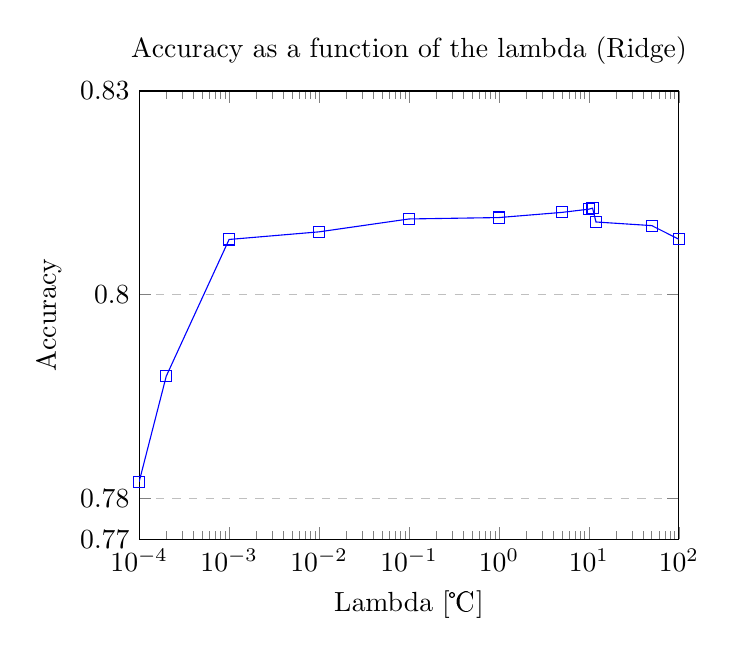
\begin{tikzpicture}
\begin{axis}[
    title={Accuracy as a function of the lambda (Ridge)},
    xlabel={Lambda [\textcelsius]},
    ylabel={Accuracy},
    xmode=log,
    xmin=0.0001, xmax=100,
    ymin=0.77, ymax=0.825,
    xtick={0.0001,0.001,0.01,0.1,1,10,100},
    ytick={0.77,0.775, 0.8,0.825},
    legend pos=north west,
    ymajorgrids=true,
    grid style=dashed,
]

\addplot[
    color=blue,
    mark=square,
    ]
    coordinates {
    (0.0001,0.77706)(0.0002,0.79)(0.001,0.80678)(0.01,0.807715)(0.1,0.809295)(1,0.809468)(5,0.8101)(10,0.810496)(11,0.810624)(12,0.808924)(50,0.80848)(100, 0.806816)
    };
    \legend{}
    
\end{axis}
\end{tikzpicture}

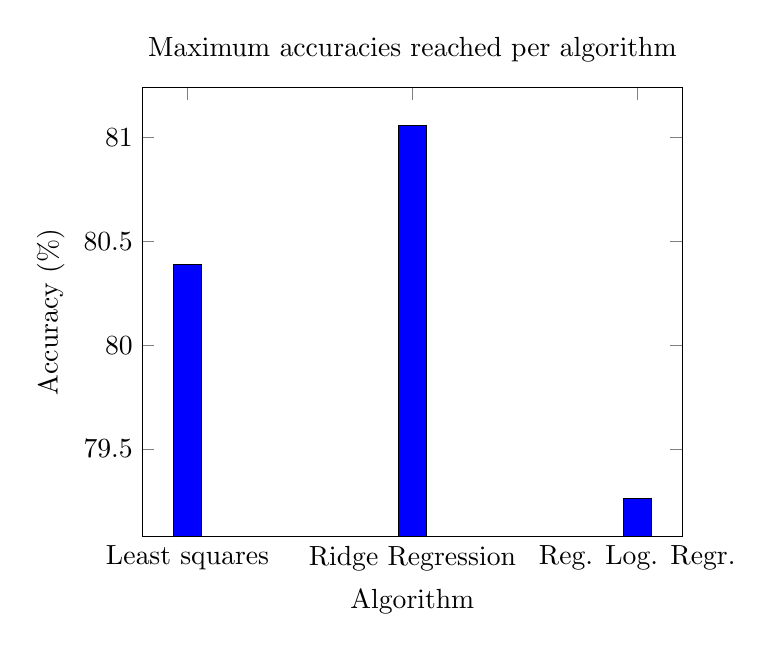
\begin{tikzpicture}
\begin{axis}[
title={Maximum accuracies reached per algorithm},
    symbolic x coords={ Least squares, Ridge Regression, Reg. Log. Regr.},
    xtick=data,
    xlabel={Algorithm},
    ylabel={Accuracy (\%)}]
    \addplot[ybar,fill=blue] coordinates {
        (Least squares,80.39)
        (Ridge Regression,81.06)
        (Reg. Log. Regr.,79.26)
    };
\end{axis}
\end{tikzpicture}

\end{document}
